\documentclass[aspectratio=169,13pt,t] {beamer}
%
% Choose how your presentation looks.
%
% For more themes, color themes and font themes, see:
% http://deic.uab.es/~iblanes/beamer_gallery/index_by_theme.html
%
\mode<presentation>
{
  \usetheme{Madrid}      % or try Darmstadt, Madrid, Warsaw, ...
  \usecolortheme{beaver} % or try albatross, beaver, crane, ...
  \usefonttheme{serif}  % or try serif, structurebold, ...
%  \setbeamertemplate{navigation symbols}{}
  \setbeamertemplate{caption}[numbered]
  \setbeamertemplate{items}[default]
}

\usepackage[,UTF8,linespread=1.2]{ctex}
\usepackage{wrapfig}
\usepackage{caption}
\captionsetup[figure]{name=图,labelsep=period}
\usepackage[,most]{tcolorbox}
\usepackage{picinpar}


\usepackage{xcolor}
\definecolor{xy_blue}{cmyk}{0.6,0.35,0.0,0.4}
\definecolor{xy_orange}{cmyk}{0.0,0.7,1.0,0.0}
\definecolor{xy_green}{cmyk}{0.2,0.0,1.0,0.15}
\xdefinecolor{xy_gold}{RGB}{135,103,79}
\xdefinecolor{xy2_gold}{cmyk}{0,0.35,0.75,0.05}


\setbeamercolor{section number projected}{fg=red,bg=red!20}%控制球的颜色
\setbeamercolor{subsection number projected}{fg=blue,bg=blue!40}
\setbeamercolor{item}{fg=xy_gold} %设置列表项颜色

\usepackage{amsthm}
\newtheorem{peroration}{结论：}
\newtheorem{exploration}{探究：}
\newtheorem{prooft}{证明：}
\newtheorem{question}{问题}
\newtheorem*{solve}{解:}
\newtheorem{instance}{例}   % 解：独立计数器
\BeforeBeginEnvironment{peroration}{%
	\setbeamercolor{block title}{bg=xy_green,fg=white}
	\setbeamercolor{block body}{bg=xy_green!10}
}
\AfterEndEnvironment{peroration}{
	\setbeamercolor{block title}{bg=xy_blue,fg=white}
	\setbeamercolor{block body}{bg=xy_blue!10}
}
\BeforeBeginEnvironment{exploration}{%
	\setbeamercolor{block title}{bg=xy_orange,fg=white}
	\setbeamercolor{block body}{bg=xy_orange!10}
}
\AfterEndEnvironment{peroration}{
	\setbeamercolor{block title}{bg=xy_blue,fg=white}
	\setbeamercolor{block body}{bg=xy_blue!10}
}
\BeforeBeginEnvironment{solution}{%
	\setbeamercolor{block title}{bg=xy_green,fg=white}
	\setbeamercolor{block body}{bg=xy_green!10}
}
\AfterEndEnvironment{solution}{
	\setbeamercolor{block title}{bg=xy_green,fg=white}
	\setbeamercolor{block body}{bg=xy_green!10}
}
\BeforeBeginEnvironment{prooft}{%
	\setbeamercolor{block title}{bg=xy_green,fg=white}
	\setbeamercolor{block body}{bg=xy_green!10}
}
\AfterEndEnvironment{prooft}{
	\setbeamercolor{block title}{bg=xy_green,fg=white}
	\setbeamercolor{block body}{bg=xy_green!10}
}
\BeforeBeginEnvironment{question}{%
	\setbeamercolor{block title}{bg=xy_orange,fg=white}
	\setbeamercolor{block body}{bg=xy_orange!10}
}
\AfterEndEnvironment{question}{
	\setbeamercolor{block title}{bg=xy_green,fg=white}
	\setbeamercolor{block body}{bg=xy_green!10}
}
\BeforeBeginEnvironment{solve}{%解：
	\begingroup
	\setbeamercolor{block title}{bg=xy_orange!60,fg=white}
	\setbeamercolor{block body}{bg=xy_orange!10}
}
\AfterEndEnvironment{solve}{%解：
	\endgroup
}

\setbeamercolor{prooft}{fg=red, bg=green!10}       % 标题颜色
\setbeamercolor{prooft body}{fg=red, bg=red!5}  % 内容块背景
\setbeamerfont{prooft head}{series=\bfseries}       % 标题字体
\setbeamerfont{question body}{shape=\upshape}         % 内容字体
\renewcommand{\thefigure}{\arabic{figure}}

\newtcolorbox{summarybox}[1][]{
	colback=purple!10,
	colframe=purple!70!black,
	fonttitle=\bfseries,
	title=#1,
	arc=1mm,
	boxrule=0pt,drop shadow,
	left=2mm, right=2mm, top=2mm, bottom=2mm,
}
\newtcolorbox{summarybox-answer}{
	width=0.9\textwidth,
	colback=white,
	blanker,
	borderline west={2pt}{20pt}{cyan},
	left=10mm, right=2mm, top=2mm, bottom=2mm,
	}
\title[3.4函数的应用（一）]{3.4 函数的应用（一）}
\subtitle{用一次函数、二次函数、幂函数模型解决实际问题}
\author[好好学习，努力向上]{}
\institute{}
\date{2026.10.29}
%\setbeamertemplate{theorems}[numbered]
\theoremstyle{definition}
\newtheorem{exam}{例}
\AtBeginSection[]
{
  \begin{frame}<beamer>
    \frametitle{本节主要内容}
    \tableofcontents[currentsection,currentsubsection]
  \end{frame}
}

\AtBeginDocument{
	\setlength{\abovedisplayskip}{3pt}
	\setlength{\belowdisplayskip}{3pt}
	\setbeamertemplate{theorems}[numbered]
}

\usepackage{pgfplots}
\pgfplotsset{compat=1.18}
\usetikzlibrary{arrows.meta}

\begin{document}
\begin{frame}{}
	\titlepage
\end{frame}

\begin{frame}{内容概览}
	\tableofcontents
\end{frame}

\section{个税问题}

	\begin{frame}{个税问题}
	\textbf{例1} 设小王的专项扣除比例、专项附加扣除金额、依法确定的其他扣除金额与 3.1.2 例8相同，全年综合所得收入额为 \(x\)（单位：元），应缴纳综合所得个税税额为 \(y\)（单位：元）.
	\begin{itemize}
		\item （1）求 \(y\) 关于 \(x\) 的函数解析式；
		\item （2）如果小王全年的综合所得由 \(117\,600\) 元增加到 \(153\,600\) 元，那么他全年应缴纳多少综合所得个税？
	\end{itemize}
	
	\vspace{0.5em}
%	\textbf{分析：}根据 3.1.2 例8中公式②，可得应纳税所得额 \(t\) 关于综合所得收入额 \(x\) 的解析式 \(t=g(x)\)，再结合 \(y=f(t)\) 的解析式③，即可得出 \(y\) 关于 \(x\) 的函数解析式.
\end{frame}

\begin{frame}{解：（1）求函数解析式}
	\textbf{解：}（1）由个人应纳税所得额计算公式，可得
	\begin{align*}
		t &= x - 60\,000 - x(8\% + 2\% + 1\% + 9\%) - 9\,600 - 560 \\
		&= 0.8x - 70\,160.
	\end{align*}
	令 \(t=0\)，得 \(x=87\,700\).
	
	根据个人应纳税所得额的规定可知，当 \(0 \leqslant x \leqslant 87\,700\) 时，\(t=0\). 所以，个人应纳税所得额 \(t\) 关于综合所得收入额 \(x\) 的函数解析式为
	\[
	t = \begin{cases}
		0, & 0 \leqslant x \leqslant 87\,700, \\
		0.8x - 70\,160, & x > 87\,700.
	\end{cases}
	\]
\end{frame}

\begin{frame}{求函数解析式（续）}
	结合 3.1.2 例8 的解析式③，可得：
	\small
	\begin{itemize}
		\item 当 \(0 \leqslant x \leqslant 87\,700\) 时，\(t=0\)，所以 \(y=0\)；
		\item 当 \(87\,700 < x \leqslant 132\,700\) 时，\(0 < t \leqslant 36\,000\)，所以 \\ \(y = t \times 3\% = 0.024x - 2\,104.8\)；
		\item 当 \(132\,700 < x \leqslant 267\,700\) 时，\(36\,000 < t \leqslant 144\,000\)，所以 \\ \(y = t \times 10\% - 2\,520 = 0.08x - 9\,536\)；
		\item 当 \(267\,700 < x \leqslant 462\,700\) 时，\(144\,000 < t \leqslant 300\,000\)，所以 \\ \(y = t \times 20\% - 16\,920 = 0.16x - 30\,952\)；
		\item 当 \(462\,700 < x \leqslant 612\,700\) 时，\(300\,000 < t \leqslant 420\,000\)，所以 \\ \(y = t \times 25\% - 31\,920 = 0.2x - 49\,460\)；
	\end{itemize}
\end{frame}

\begin{frame}{求函数解析式（续）}
	\small
	\begin{itemize}
		\item 当 \(612\,700 < x \leqslant 912\,700\) 时，\(420\,000 < t \leqslant 660\,000\)，所以 \\ \(y = t \times 30\% - 52\,920 = 0.24x - 73\,968\)；
		\item 当 \(912\,700 < x \leqslant 1\,287\,700\) 时，\(660\,000 < t \leqslant 960\,000\)，所以 \\ \(y = t \times 35\% - 85\,920 = 0.28x - 110\,476\)；
		\item 当 \(x > 1\,287\,700\) 时，\(t > 960\,000\)，所以 \\ \(y = t \times 45\% - 181\,920 = 0.36x - 213\,492\).
	\end{itemize}
	
	
\end{frame}

\begin{frame}{函数解析式}
	所以，函数解析式为
	\begin{equation}
		y = \begin{cases}
			0, & 0 \leqslant x \leqslant 87\,700, \\
			0.024x - 2\,104.8, & 87\,700 < x \leqslant 132\,700, \\
			0.08x - 9\,536, & 132\,700 < x \leqslant 267\,700, \\
			0.16x - 30\,952, & 267\,700 < x \leqslant 462\,700, \\
			0.2x - 49\,460, & 462\,700 < x \leqslant 612\,700, \\
			0.24x - 73\,968, & 612\,700 < x \leqslant 912\,700, \\
			0.28x - 110\,476, & 912\,700 < x \leqslant 1\,287\,700, \\
			0.36x - 213\,492, & x > 1\,287\,700.
		\end{cases} \tag{④}
	\end{equation}
\end{frame}



\begin{frame}{解：（2）计算个税}
	\textbf{（2）}根据④，当 \(x=153\,600\) 时，
	\[
	y = 0.08 \times 153\,600 - 9\,536 = 2\,752.
	\]
	所以，小王全年需要缴纳的综合所得个税税额为 \(2\,752\) 元.
	
	\vspace{1em}
	根据个人收入情况，利用上面获得的个税和综合所得收入关系的函数解析式，就可以直接求得应缴纳的个税.
\end{frame}
\section{路程问题：分段函数模型}

\begin{frame}{例2：汽车行驶的平均速率与时间}
	\begin{exam}
		一辆汽车在某段路程中行驶的平均速率 $v$（km/h）与时间 $t$（h）的关系如图 3.4-1 所示.
		\begin{enumerate}[(1)]
			\item 求图中阴影部分的面积，并说明其实际含义；
			\item 里程表出发前读数为 $2\,004$ km，建立里程表读数 $s$（km）与时间 $t$ 的函数解析式，并画出图象.
		\end{enumerate}
	\end{exam}
\end{frame}

\begin{frame}{图 1：速率 $v$ 随时间 $t$ 的变化}
	\begin{center}
	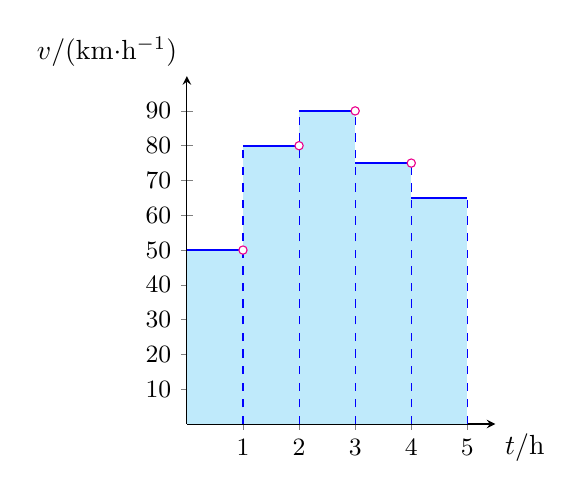
\begin{tikzpicture}
		\begin{axis}[
			width=5.5cm, height=6cm,
			xmin=0, xmax=5.5, ymin=0, ymax=100,
			axis lines=middle, axis line style={->},
			xlabel={$t$/h}, ylabel={$v$/(km$\cdot$h$^{-1}$)},
			xlabel style={below right}, ylabel style={above left},
			xtick={0,1,2,3,4,5}, ytick={10,20,...,90},
			tick label style={font=\small},
			>=stealth,
		]
		\draw[draw=none,fill=cyan!25] (0,0) rectangle (1,50);
		\draw[draw=none,fill=cyan!25] (1,0) rectangle (2,80);
		\draw[draw=none,fill=cyan!25] (2,0) rectangle (3,90);
		\draw[draw=none,fill=cyan!25] (3,0) rectangle (4,75);
		\draw[draw=none,fill=cyan!25] (4,0) rectangle (5,65);
		\addplot[const plot,jump mark left,mark=none, blue, thick,] coordinates {
				(0,50)(1,50)(1,80)(2,80)(2,90)(3,90)(3,75)(4,75)(4,65)(5,65)};
		\draw (0,0) -- (0,50);
		\draw [blue,dashed] (1,0) -- (1,80);
		\draw [blue,dashed] (2,0) -- (2,90);
		\draw [blue,dashed](3,0) -- (3,90);
		\draw [blue,dashed](4,0) -- (4,75);
		\draw [blue,dashed](5,0) -- (5,65);
		\draw[magenta,fill=white] (1,50) circle(1.5pt);
		\draw[magenta,fill=white] (2,80) circle(1.5pt);
		\draw[magenta,fill=white] (3,90) circle(1.5pt);
		\draw[magenta,fill=white] (4,75) circle(1.5pt);
		
		\end{axis}
	\end{tikzpicture}\hspace{1em}
	\captionof{figure}{}
		
	\end{center}
	在 $[0,1),[1,2),[2,3),[3,4),[4,5]$ 内速率分别为 $50,80,90,75,65$ km/h.
\end{frame}

\begin{frame}{例2（1）：阴影部分的面积}
	\begin{solve}
		阴影部分是 $5$ 个小矩形，每个宽为 $1$ h，其面积为
		\[
			50\times1+80\times1+90\times1+75\times1+65\times1=360.
		\]
	\end{solve}
	\vspace{0.8em}
	\begin{summarybox-answer}
		\textbf{实际含义}：矩形面积 $=$ 平均速率 $\times$ 时间 $=$ 路程.
		故阴影面积 $360$ 表示汽车在这 $5$ h 内行驶的路程为 \textbf{$360$ km}.
	\end{summarybox-answer}
\end{frame}

\begin{frame}{例2（2）：建立里程表读数 $s$ 与时间 $t$ 的函数}
	\begin{solve}
		每个时间段内路程与时间的关系不同，需\textbf{分段}表述：
		\[
			s=\begin{cases}
				50t+2\,004,             & 0\le t<1,\\
				80(t-1)+2\,054,         & 1\le t<2,\\
				90(t-2)+2\,134,          & 2\le t<3,\\
				75(t-3)+2\,224,          & 3\le t<4,\\
				65(t-4)+2\,299,          & 4\le t\le5.
			\end{cases}
		\]
		（各段起点累计里程：$2054,2134,2224,2299$，终点 $2364=2004+360$.）
	\end{solve}
\end{frame}

\begin{frame}{图 2：里程表读数 $s$ 随时间 $t$ 的变化}
	\begin{center}
	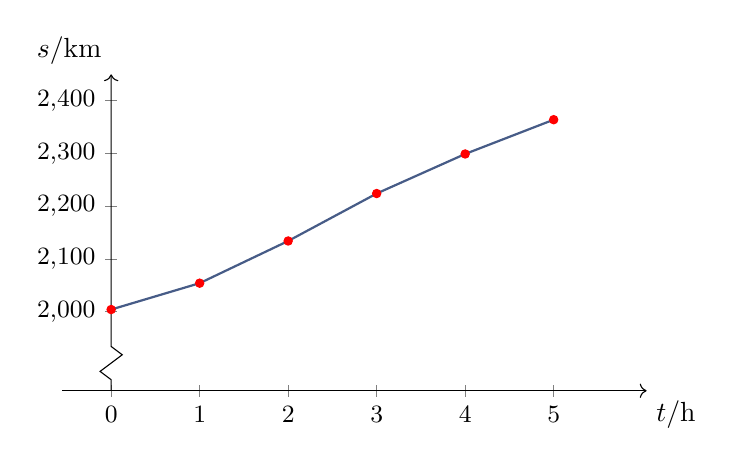
\begin{tikzpicture}
		\begin{axis}[
			clip=false,
			width=9cm, height=5.6cm,
			xmin=0, xmax=5.5, ymin=1900, ymax=2400,
			axis lines=middle, axis line style={->},
			xlabel={$t$/h}, ylabel={$s$/km},
			xlabel style={below right}, ylabel style={above left},
			xtick={0,1,2,3,4,5}, ytick={2000,2100,2200,2300,2400},
			tick label style={font=\small},
			axis y discontinuity=crunch,
			enlargelimits=true,	
			hide obscured x ticks=false,	%不遮挡x轴刻度。
		]
		\addplot[xy_blue, thick,] coordinates {
			(0,2004)(1,2054)(2,2134)(3,2224)(4,2299)(5,2364)};
		\addplot[only marks,red, mark=*, mark size=1.5pt,] coordinates {
	(0,2004)(1,2054)(2,2134)(3,2224)(4,2299)(5,2364)};
		\end{axis}
	\end{tikzpicture}
	\captionof{figure}{}
	\end{center}
\end{frame}

\begin{frame}{分段函数建模小结}
	\begin{summarybox}[方法]
	\begin{enumerate}
		\item 不同区间内对应规律不同时，用\textbf{分段函数}表示；
		\item 注意每一段\textbf{端点}的归属，保证函数在各段衔接；
		\item \textbf{函数图象}对分析题意很有帮助，要提高读图能力.
	\end{enumerate}
	\end{summarybox}
	\vspace{1em}
	\begin{summarybox-answer}
		现实问题中经常用到分段函数（如出租车计费、阶梯水价、个税等）.
	\end{summarybox-answer}
\end{frame}

\section{幂函数与二次函数模型}

\begin{frame}{例：汽车紧急刹车距离 $y=ax^{2}$}
	\begin{exam}
		用模型 $y=ax^{2}$ 描述刹车后滑行距离 $y$（m）与车速 $x$（km/h）的关系.
		某型车在 $60$ km/h 时滑行 $20$ m. 若限速 $100$ km/h 的公路上该车刹车距离为 $50$ m，它是否超速？
	\end{exam}
	\pause
	\begin{solve}
		代入 $x=60,\ y=20$：$20=a\cdot60^{2}$，得 $a=\dfrac{20}{3600}=\dfrac{1}{180}$.
		于是 $y=\dfrac{x^{2}}{180}$. 当 $x=100$ 时，
		\[
			y=\frac{100^{2}}{180}\approx55.6\ \text{m}.
		\]
	\end{solve}
\end{frame}

\begin{frame}{刹车距离模型（续）}
	\begin{columns}
		\column{0.55\textwidth}
		\begin{tikzpicture}[baseline=(current bounding box.north)]
			\begin{axis}[
				width=7.5cm, height=5.5cm,
				xmin=0, xmax=110, ymin=0, ymax=65,
				axis lines=middle, axis line style={->},
				xlabel={$x$/(km/h)}, ylabel={$y$/m},
				xlabel style={below right}, ylabel style={above left},
				tick label style={font=\small},
			]
			\addplot[domain=0:110, samples=100, thick, xy_orange] {x^2/180};
			\addplot[only marks, mark=*, color=xy_green!70!black] coordinates {(60,20)(100,55.6)};
			\end{axis}
		\end{tikzpicture}
		\captionof{figure}{$y=\dfrac{x^{2}}{180}$}
		\column{0.42\textwidth}
		\begin{summarybox}[结论]
			$100$ km/h 时正常应滑行约 $55.6$ m，
			而该车实际滑行 $50$ m $<55.6$ m，
			说明实际车速\textbf{小于} $100$ km/h.
		\end{summarybox}
		\begin{summarybox-answer}
			故该车\textbf{未超速}.
		\end{summarybox-answer}
	\end{columns}
\end{frame}

\begin{frame}{例：周长一定的矩形广告牌，何时面积最大？}
	\begin{exam}
		某广告公司要为客户设计一幅周长为 $l$（m）的矩形广告牌，如何设计长与宽，可使广告牌面积最大？
	\end{exam}
	\pause
	\begin{solve}
		设一边长为 $x$，则邻边长为 $\dfrac{l}{2}-x$，面积
		\[
			S=x\left(\frac{l}{2}-x\right)=-x^{2}+\frac{l}{2}x.
		\]
		这是开口向下的二次函数，当 $x=\dfrac{l}{4}$ 时取最大值 $S_{\max}=\dfrac{l^{2}}{16}$.
	\end{solve}
\end{frame}

\begin{frame}{面积最大问题（续）}
	\vspace{-2em}
	\begin{summarybox}[结论]
		当矩形的长、宽都等于 $\dfrac{l}{4}$，即广告牌设计为\textbf{正方形}时，
		面积最大，最大面积为 $\dfrac{l^{2}}{16}\ \mathrm{m^{2}}$.
	\end{summarybox}
	\vspace{1em}
	\begin{columns}
		\column{0.1\textwidth}
%		\begin{tikzpicture}
%			\begin{axis}[
%				width=7.5cm, height=5cm,
%				xmin=0, xmax=1, ymin=0, ymax=0.28,
%				axis lines=middle, axis line style={->},
%				xlabel={$x$}, ylabel={$S$},
%				xlabel style={below right}, ylabel style={above left},
%				tick label style={font=\small},
%			]
%			\addplot[domain=0:1, samples=100, thick, xy_green!70!black] {x*(0.5-x)};
%			\end{axis}
%		\end{tikzpicture}
%		\captionof{figure}{取 $l=2$，$S=x(0.5-x)$}
		\column{0.9\textwidth}
		\begin{summarybox-answer}
			周长固定时，\textbf{正方形}面积最大——二次函数最值的典型应用.
		\end{summarybox-answer}
	\end{columns}
\end{frame}

\section{课堂练习与作业}

\begin{frame}{课堂练习：阶梯水价}
	\begin{question}
		某市居民生活用水实行“阶梯水价”：
		不超过 $12\ \mathrm{m^{3}}$ 部分 $3$ 元/$\mathrm{m^{3}}$；
		超过 $12$ 不超过 $18\ \mathrm{m^{3}}$ 部分 $6$ 元/$\mathrm{m^{3}}$；
		超过 $18\ \mathrm{m^{3}}$ 部分 $9$ 元/$\mathrm{m^{3}}$.
		某户本月交水费 $48$ 元，求本月用水量.
	\end{question}
	\pause
	\begin{solve}
		用水 $12\ \mathrm{m^{3}}$ 时水费 $=12\times3=36$ 元 $<48$；
		用水 $18\ \mathrm{m^{3}}$ 时水费 $=36+6\times6=72$ 元 $>48$.
		故用水量在 $(12,18)$ 之间，设用水 $x$：$36+6(x-12)=48$，得 $x=14\ \mathrm{m^{3}}$.
	\end{solve}
\end{frame}



\begin{frame}{本节小结}
	\begin{summarybox}[函数应用（一）要点]
	\begin{enumerate}
		\item 实际问题 $\rightarrow$ 建立\textbf{函数模型}（一次、二次、幂函数、分段函数）；
		\item 分段函数要\textbf{分段列式、注意端点}；
		\item 二次函数可求\textbf{最大值/最小值}（最优化问题）；
		\item 画函数图象帮助理解和检验结果.
	\end{enumerate}
	\end{summarybox}
\end{frame}


\begin{frame}{课后作业}
	
	P95练习 1---3
	
	P96习题3.4 1---5
%	\begin{summarybox}[习题 3.4] \quad 1---5
%		%	\begin{enumerate}
%			%		\item 汽车以 $60$ km/h 从 A 到 $150$ km 外的 B 地，停留 $1$ h 后以 $50$ km/h 返回.
%			%		      把车与 A 地距离 $x$、车速 $v$ 分别表示为时间 $t$ 的函数并画图象；
%			%		\item 建造容积 $1\,200\ \mathrm{m^{3}}$、深 $6$ m 的无盖蓄水池，池壁造价 $95$ 元/$\mathrm{m^{2}}$、
%			%		      池底 $135$ 元/$\mathrm{m^{2}}$，如何设计长与宽使总造价控制在 $7$ 万元以内；
%			%		\item 弹簧伸长长度 $x$ 与拉力 $F$ 近似成正比例关系，根据所给数据求一个函数解析式.
%			%	\end{enumerate}
%	\end{summarybox}
\end{frame}

\end{document}
